\section{\coolname{}}
\label{sec:approach}


\label{subsec:approach_overview}

\coolname is an end-to-end model that takes as input $N$ RGB images $\hat{\mathcal{I}} \!=\! (\hat{I}_i)_{i=1}^N$ and optional geometric inputs corresponding to all or a subset of the input views:
\begin{enumerate}[label=(\textbf{\alph*})]
\item %
generic central camera calibrations \cite{GrossN2001,VasilGAPBSG2020,ZhangLKYRT2024} as ray directions $\hat{\mathcal{R}} \!=\! (\hat{R}_i)_{i \in S_\text{r}}$,

\item %
poses in the frame of the first view $\hat{I}_1$ as quaternions $\hat{\mathcal{Q}} \!=\! (\hat{Q}_i)_{i \in S_\text{q}}$ and translations $\hat{\mathcal{T}} \!=\! (\hat{T}_i)_{i \in S_\text{t}}$, and

\item %
ray depth for each pixel $\hat{\mathcal{D}} \!=\! (\hat{D}_i)_{i \in S_\text{d}}$,
\end{enumerate}
where $S_\text{r}, S_\text{q}, S_\text{t}, S_\text{d}$ are subsets of frame indices $[1, N]$.


\coolname maps these inputs to an $N$-view factored metric 3D output (as shown in \cref{fig:method}):
\begin{equation}
    \label{eq:MapAnything}
    \!f_\text{MapAnything}\bigl(\hat{\mathcal{I}}, [\hat{\mathcal{R}}, \hat{\mathcal{Q}}, \hat{\mathcal{T}}, \hat{\mathcal{D}}] \bigr)
    \!=\! \{m, (R_i, \uts{D}_i, \uts{P}_i)_{i=1}^N) \}
     \text{,}  
\end{equation}
where $m \!\in\! \R$ is the predicted global metric scaling factor, and for each view $i$,
$R_i \!\in\! \R^{3 \times H \times W}$ are the predicted local ray directions,
$\uts{D}_i \!\in\! \R^{1 \times H \times W}$ are the ray depths in a up-to-scale space (indicated by the tilde),
and $\uts{P}_i \!\in\! \R^{4 \times 4}$ is the pose of image $\hat{I}_i$ in the frame of image $\hat{I}_1$, represented as quaternion $Q_i$
and up-to-scale translation $\uts{T}_i \!\in\! \R^3$.
We can further use this factored output to get the up-to-scale local pointmaps (3D points corresponding to each pixel) as $\uts{L}_i \!=\! R_i \!\cdot\! \uts{D}_i \!\in\! \R^{3 \times H \times W}$.
Then, leveraging the rotation matrix ${O}_i$ 
(obtained from $Q_i$) and up-to-scale translation, we can compute the $N$-view up-to-scale pointmaps in world frame as $\uts{X}_i \!=\! {O}_i \!\cdot\! \uts{L}_i \!+\! \uts{T}_i$.
The final metric 3D reconstruction for the $N$ input views (in the frame of image $I_1$) is given by
$\metric{X}_i \!=\! m \!\cdot\! \uts{X}_i$ for $i \!\in\! [1, N]$.



\subsection{Encoding Images \& Geometric Inputs}

Given $N$ visual inputs and optional dense geometric inputs, we first encode them into a common latent space.
For images, we use DINOv2 (Apache 2.0) \cite{OquabDMVSKFHMEABGHHLMRSSXJMLJB2024}.
Among a wide variety of pre-trained options, such as CroCov2 \cite{WeinzLLCABCACR2023}, DUSt3R's image encoder \cite{WangLCCR2024}, RADIO \cite{RanziHKM2024, HeinrRHLKTCM2025}, and random-init linear patchification, we find DINOv2 to be optimal in terms of downstream performance, convergence speed, and generalization (especially when fine-tuned with a small learning rate). 
We use the $24$th layer normalized patch features from DINOv2 ViT-G, $F_\text{I} \!\in\! \R^{1536 \times H/14 \times W/14}$.

\coolname can also encode other geometric quantities.
Before feeding these geometric quantities to our network, we factorize them to enable training and inference across both metric and up-to-scale quantities.
To support use cases where only rotation or translation might be individually present (for e.g., IMU \& GPS priors) and to deal with the entanglement of translation with scale, we encode rotation and translation separately.
Furthermore, since we don't assume depth \& pose to always be provided together as input, we decouple their normalization (note that this is separate from the training objective where we normalize predicted depth \& pose together since we want multi-view consistency).

In particular, when provided, the ray depths are first decoupled into average per-view depth $\hat{z}_{di} \!\in\! \R^+$ and normalized ray depths $\hat{D}_i / \hat{z}_{di}$.
Furthermore, when translations $\hat{\mathcal{T}}$ are provided, \coolname computes the pose scale as the average distance to the world frame, %
$\hat{z}_\text{p} \!=\! \frac{1}{\abs{S_t}} \sum_{i\in{S_t}} \lVert \hat{T}_i \rVert$.
This pose scale is used as the same input for all frames with input translation and is also used to get the normalized translations $\hat{T}_i / \hat{z}_\text{p}$.
Since we are interested in effectively exploiting the metric scale information from geometric inputs, \coolname{} only uses the pose scale and depth scales when the poses and depths provided for specific frames are metric.
Furthermore, the metric scale values can be large and drastically vary across scene sizes, hence, we log-transform scales before encoding them.

We encode ray directions and normalized ray depths using a shallow convolutional encoder \cite{MouWXWZQSQ2024}, where the spatial resizing only happens once with a pixel unshuffle of size 14.
This projects the dense geometric inputs into the same spatial and latent dimension as the DINOv2 features, \ie, $F_\text{R}, F_\text{D} \!\in\! \R^{1536 \times H/14 \times W/14}$.
For the global non-pixel quantities, i.e, rotations (represented as unit quaternions), translation directions, depth and pose scales, we use a 4-layer MLP with GeLU activations to project the quantities to features $F_\text{Q}, F_\text{T}, F_{\hat{z}_d}, F_{\hat{z}_\text{p}} \!\in\! \R^{1536}$.
Once all input quantities are encoded, they are passed through layer normalization, summed together, and followed by another layer normalization to obtain the final per-view encodings for each input view.
These are then flattened into tokens $F_\text{E} \!\in\! \R^{1536 \times ({HW}/{256})}$.


We append a single learnable scale token to the set of $N$ view patch tokens and input the tokens into a multi-view transformer to allow information across multiple views to attend to each other and propagate. 
We use a 16-layer alternating-attention transformer \cite{WangCKVRN2025} with 24~heads of multi-headed attention, a latent dimension of 1536 and an MLP ratio of 4, initialized using the last 16 layers of DINOv2 ViT-G \cite{oquab2023dinov2, lin2025depth}.
To distinguish the reference view (i.e., the first one), we add a constant reference view embedding to the set of patch tokens corresponding to view $I_{1}$.
For simplicity, we do not use Rotary Positional Embedding (RoPE) \cite{SuLPMWL2024}.
We find that the patch-level positional encoding from DINOv2 suffices, and RoPE leads to unnecessary biases, given that it was originally applied in every attention layer.

\subsection{Factored Scene Representation Prediction}

Once the multi-view transformer fuses information across different views and outputs the $N$-view patch tokens and scale token, \coolname{} further decodes these tokens into factored quantities representing the metric 3D geometry.
In particular,
we use a DPT head \cite{RanftBK2021} to decode the $N$-view patch tokens into $N$ dense per-view outputs, \ie, ray directions $R_i$ (normalized to unit length), up-to-scale ray depths $\uts{D}_i$,
masks $M_i$ representing non-ambiguous classes for depth,
and world-frame pointmap confidence maps $C_i$.
Furthermore, we input the $N$-view patch tokens into an average pooling-based convolutional pose head \cite{ChenCPB2024} to predict the unit quaternions $Q_i$ and up-to-scale translations $\uts{T}_i$.
Finally, the scale token is passed through a 2-layer MLP with ReLU activations to predict the metric scaling factor.
Since the metric scale of a scene can vary vastly, we exponentially scale the prediction to obtain the metric scaling factor $m$.
As shown in \cref{tab:ablation_rep}, we find that this decoupling of scale prediction is critical to achieving universal metric feed-forward inference.
Finally, as mentioned earlier, %
these factored predictions can be used together to obtain the metric 3D reconstruction.

\begin{figure*}[!t]
    \centering
    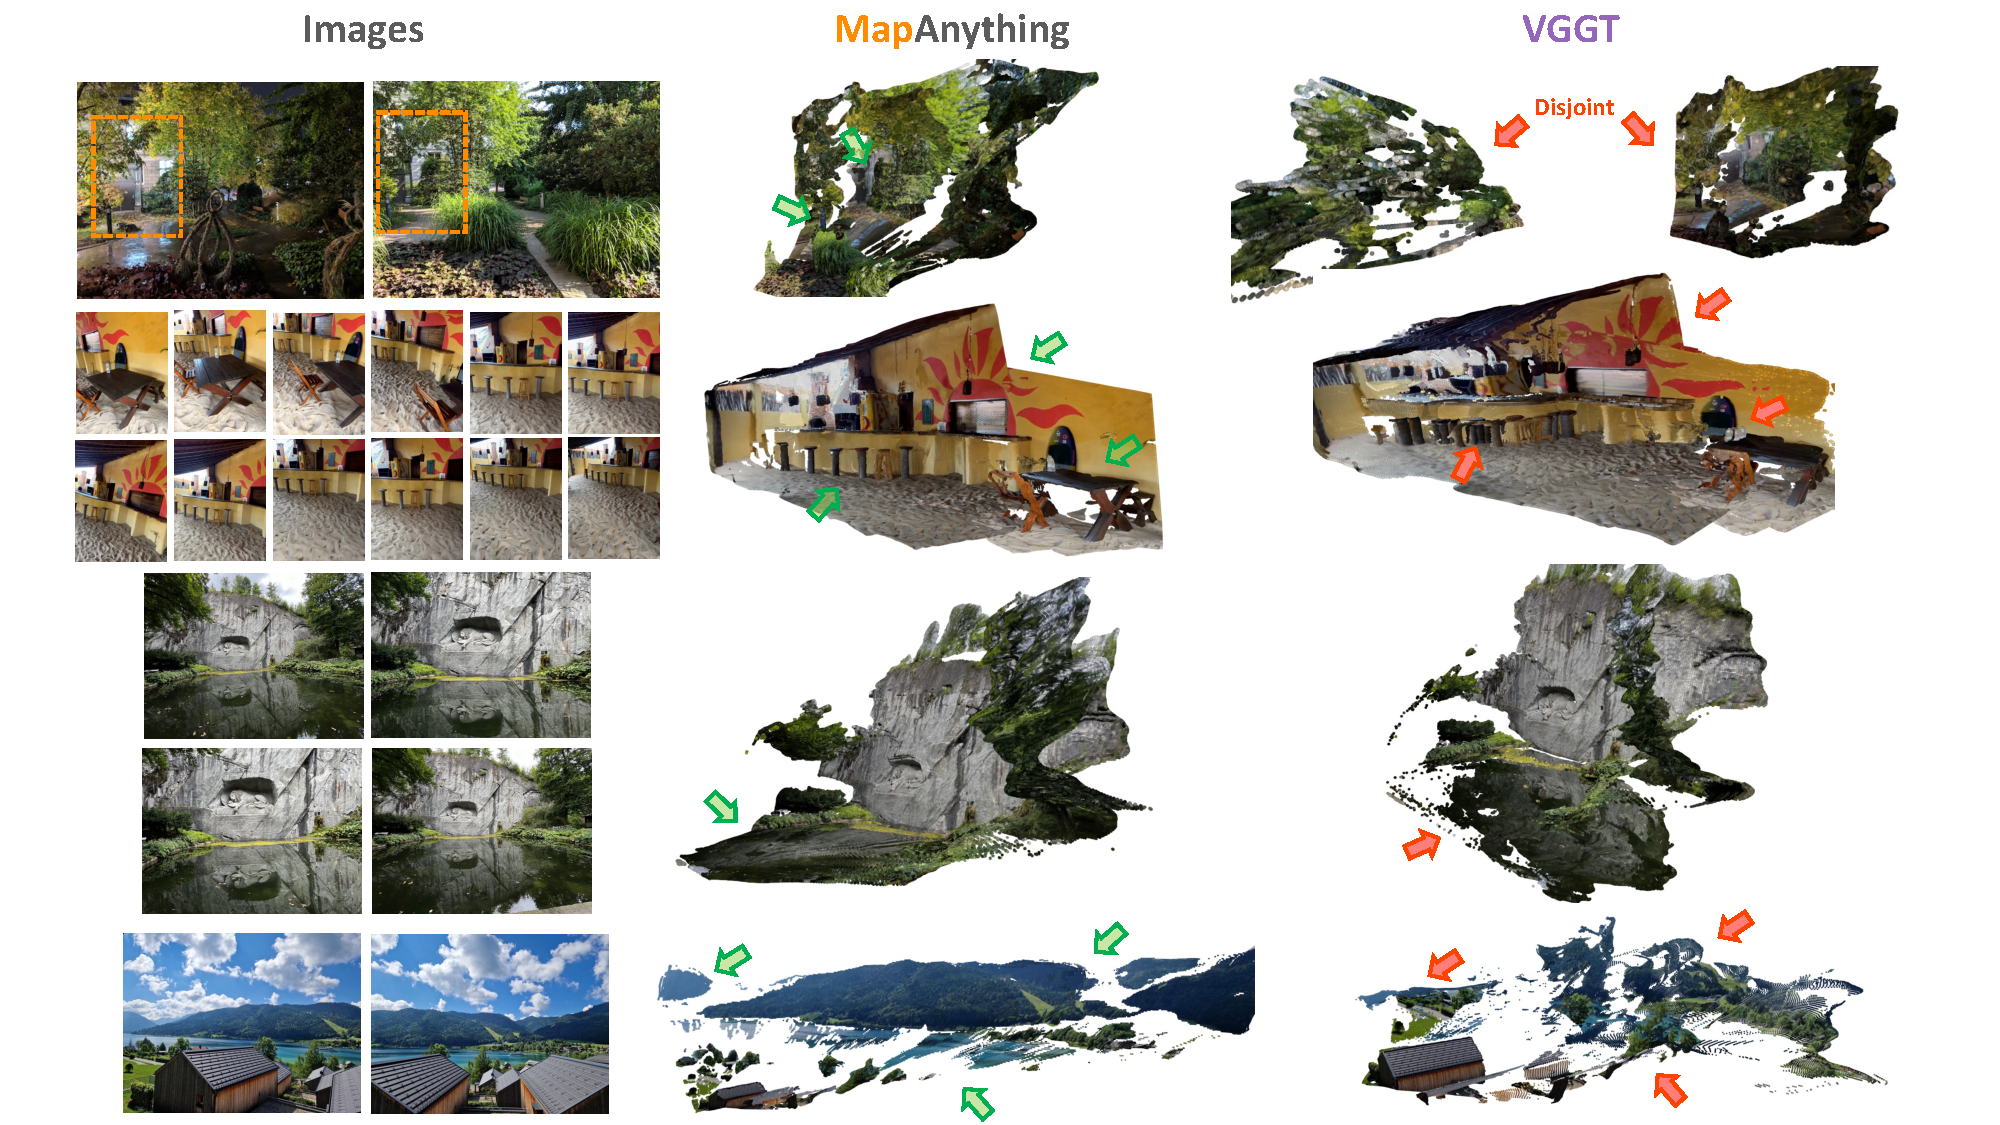
\includegraphics[trim={0cm 0.15cm 0cm 0cm},clip,width=0.94\linewidth]{figs/Qual_Comparison.pdf}
    \caption{\textbf{Qualitative comparison of \coolname to VGGT \cite{WangCKVRN2025} using only in-the-wild images as input.}
    For a fair comparison, we apply the same normal-based edge mask post-processing and our sky mask to both methods. %
    \coolname more effectively deals with large disparity changes, seasonal shifts, textureless surfaces, water bodies and large scenes.
    }
    \label{fig:qual_comparison}
\end{figure*}

\subsection{Training Universal Metric 3D Reconstruction}
\label{sec:training}

We train \coolname end-to-end using multiple losses depending on the available supervision.
Since ray directions $R_i$ and pose quaternions $Q_i$ do not depend on scene scale, their losses are:
$\mathcal{L}_\text{rays} \!=\! \sum_{i=1}^N \| \hat{R}_i \!-\! R_i \|$ and
$\mathcal{L}_\text{rot} \!=\! \sum_{i=1}^N \min(\| \hat{Q}_i \!-\! Q_i \|, \| {-}\hat{Q}_i \!-\! Q_i \|)$.
This accounts for the two-to-one mapping of unit quaternions, and the regression loss is similar to a geodesic angular distance.

For the predicted up-to-scale ray depths $\uts{D}_i$, pose translations $\uts{T}_i$, local pointmaps $\uts{L}_i$ and world frame pointmaps $\uts{X}_i$, we follow DUSt3R \cite{WangLCCR2024} and use the ground-truth validity masks $V_i$ to compute the scaling factors for the ground truth $\hat{z} \!=\! \| (\hat{X}_i[V_i])_{i=1}^{N} \| / \sum_{i=1}^N \!V_i$ and the up-to-scale predictions $\uts{z} \!=\! \| (\uts{X}_i[V_i])_{i=1}^{N} \| / \sum_{i=1}^N \!V_i$. 
Likewise, to ensure that gradients from the scale loss do not influence the geometry, we use the predicted metric scaling factor $m$ and detached up-to-scale norm scaling factor $\uts{z}$ to compute the metric norm scaling factor $\metric{z} \!=\! m \!\cdot\! \mathrm{sg}(\uts{z})$, where $\mathrm{sg}$ indicates stop-grad.


Given these scaling factors, we compute the scale-invariant translation loss as $\mathcal{L}_\text{translation} \!=\! \sum_{i=1}^N \| \hat{T}_i/\hat{z} \!-\! \uts{T}_i/\uts{z} \|$.
We find that it is critical to apply losses in log-space for ray depths, pointmaps and the metric scale factor.
Specifically, we use $f_\mathrm{log} \colon \mathbf{x} \to (\mathbf{x}/\|\mathbf{x}\|) \!\cdot\! \log(1 \!+\! \|\mathbf{x}\|)$.
Thus, the loss for the ray depths is $\mathcal{L}_\text{depth} \!=\! \sum_{i=1}^N \| f_\mathrm{log}(\hat{D}_i/\hat{z}) \!-\! f_\mathrm{log}(\uts{D}_i/\uts{z}) \|$.
Likewise, the loss for the local pointmaps is $\mathcal{L}_\text{lpm} \!=\! \sum_{i=1}^N \| f_\mathrm{log}(\hat{L}_i/\hat{z}) \!-\! f_\mathrm{log}(\uts{L}_i/\uts{z}) \|$.
We exclude the top 5\% of per-pixel loss values to ignore imperfections and potential outliers in the training data.
Similar to DUSt3R, we add $\mathcal{L}_\text{pointmap} \!=\! \sum_{i=1}^N (C_i \| f_\mathrm{log}(\hat{X}_i/\hat{z}) \!-\! f_\mathrm{log}(\uts{X}_i/\uts{z}) \| \!-\! \alpha \log(C_i))$ as a confidence-weighted pointmap loss.
Lastly, the factored metric scale loss is given by $\mathcal{L}_\text{scale} \!=\! \| f_\mathrm{log}(\hat{z}) \!-\! f_\mathrm{log}(\metric{z}) \|$.

To capture fine details, %
we also employ a normal loss $\mathcal{L}_\text{normal}$ \cite{WangXDXDTY2025} on the local pointmaps, and a multi-scale gradient matching loss $\mathcal{L}_\text{GM}$ \cite{RanftLHSK2022, YangKHZXFZ2024} on the log of the $z$-depth in the local pointmaps.
Since the geometry from real datasets can be coarse and noisy, we apply the $\mathcal{L}_\text{normal}$ and $\mathcal{L}_\text{GM}$ losses only to synthetic datasets.
For the predicted non-ambiguous class masks, we use a binary cross entropy loss ($\mathcal{L}_\text{mask}$).

\noindent Overall, we use the following total loss: 
\begin{equation}
\begin{split}
    \label{eq:training_loss}
    \mathcal{L}
    =
    &10 \cdot \mathcal{L}_\text{pointmap}
    + \mathcal{L}_\text{rays}
    + \mathcal{L}_\text{rot}
    + \mathcal{L}_\text{translation}
    + \mathcal{L}_\text{depth}
    \\
    &+ \mathcal{L}_\text{lpm}
    + \mathcal{L}_\text{scale}
    + \mathcal{L}_\text{normal}
    + \mathcal{L}_\text{GM}
    + 0.1 \cdot \mathcal{L}_\text{mask}
\end{split}
\end{equation}
For the factored predictions, we find that up-weighting the global pointmap loss and down-weighting the mask loss is beneficial.
For all the regression losses, we use an adaptive robust loss \cite{Barro2019} (with parameters $c=0.05$ and $\alpha=0.5$) to help with robustness to outliers.

\paragraph{Training for Image \& Geometric Inputs:}
\label{para:aug_training}
To enable one-shot training of a universal model that supports various input configurations, we provide additional geometric inputs to the model with varying selection probabilities during training.
Specifically, we use an overall geometric input probability of 0.9, where each individual factorization, \ie, ray directions, ray depth, and pose, has an input probability of 0.5 each.
Whenever depth is selected as input, there is an equal probability of providing dense depth or 90\% randomly sparsified depth.
For robustness and flexibility in terms of which views have geometric information available as input, we use a per-view input probability of 0.95 and do not provide metric scale factors as input for metric-scale ground-truth datasets with a probability of 0.05.
We provide further details regarding the training setup in the supplement.

\begin{table}[b]
\caption{\label{tab:datasets}%
    \textbf{Datasets used for training and testing \coolname.}
}
\scriptsize
\centering
\newcommand{\fn}[1]{\textsuperscript{#1}}
\setlength\tabcolsep{5pt}
\begin{tabular}{llrc}
\toprule
\textbf{Dataset}                                          & \textbf{License}      & \textbf{\# Scenes} & \textbf{Metric} \\\midrule
BlendedMVS~\cite{YaoLLZRZFQ2020}                          & CC BY 4.0             &        493         & \xmark    \\
Mapillary Planet-Scale Depth~\cite{LopezGHBKK2020}                        & CC BY-NC-SA\fn{1}     &     71,428         & \tickmark \\
ScanNet++ v2~\cite{YeshwLND2023}                          & Non-commercial\fn{1}  &        926         & \tickmark \\
Spring~\cite{MehlSJNB2023}                                & CC BY 4.0             &         37         & \tickmark \\
TartanAirV2-WB~\cite{WangZWHQWHKS2020, ZhangKLJCQKJHRSW2025}     & CC BY 4.0             &         49         & \tickmark \\
UnrealStereo4K~\cite{TosiLSG2021}                         & MIT                   &          9         & \tickmark \\[.5em]
\multicolumn{4}{l}{\textbf{Additionally used for our CC BY-NC model:}} \\
Aria Synthetic Environments~\cite{AvetiXHYAPZFHOEMNB2024} & Non-commercial        &    103,890         & \tickmark \\
DL3DV-10K~\cite{LingSTZXWYGYLLSAMKKHZBB2024}              & CC BY-NC 4.0          &     10,109         & \xmark    \\
Dynamic Replica~\cite{KaraeRGNVR2023}                     & Non-commercial        &        523         & \tickmark \\
MegaDepth~\cite{LiS2018}                                  & CC BY 4.0\fn{2}       &        269         & \xmark    \\
MVS-Synth~\cite{HuangMKAH2018}                            & Non-commercial        &        120         & \tickmark \\
ParallelDomain-4D~\cite{VanHWOSLTDZV2024}                 & Non-commercial        &      1,528         & \tickmark \\
SAIL-VOS 3D~\cite{HuWYS2021}                              & Non-commercial        &        171         & \tickmark \\

\arrayrulecolor{gray}\midrule

\multicolumn{4}{l}{\textbf{Unique held-out scenes for dense up-to-N-view benchmarking:}} \\
ETH3D~\cite{SchoepSGSSPG2017}                             & CC BY-NC-SA 4.0       &         13         & \tickmark \\
ScanNet++ v2~\cite{YeshwLND2023}                          & Non-commercial\fn{1}  &         30         & \tickmark \\
TartanAirV2-WB~\cite{WangZWHQWHKS2020, ZhangKLJCQKJHRSW2025}     & CC BY 4.0             &          5         & \tickmark \\
\arrayrulecolor{black}\bottomrule
\end{tabular}\\[.2em]
\scriptsize{\fn{1} We obtained approval from the dataset owners that allows training and model release under a permissive license.
\quad
\fn{2} Crowd-sourced images with varying licenses.}
\end{table}


\paragraph{Datasets:}
We train \coolname on 13 high-quality datasets (see \cref{tab:datasets}) with diversity across indoor, outdoor, and in-the-wild scenes.
For ScanNet++ v2 and TartanAirV2-WB, we split the scenes into a training, validation, and a held-out test set, while other datasets are split into training and validation.
While MPSD is originally a monocular metric depth dataset, we acquire the pose and camera information to enable a real-world multi-view metric scale dataset with $\sim$72K scenes.
We open-sourced this MPSD metadata to enable future research.
We release two pretrained models: one licensed under Apache 2.0 trained on six datasets, and one licensed under CC BY-NC 4.0 trained on an additional seven datasets (see \cref{tab:datasets}).
We provide comparisons between both variants in the supplementary.

\paragraph{Multi-View Sampling:}
For each dataset, we exhaustively precompute the pairwise covisibility of all images in a scene using a reprojection error check based on ground-truth depth and pose.
During training, we use this precomputed covisibility with a selected covisibility threshold of 25\% to perform random walk sampling.
This enables us to sample random single-connected component graphs of covisible views that have varying coverage and mutual information.












